\documentclass[../main.tex]{subfiles}
\begin{document}

\section{Movement}
The Movement stat on a character (abbreviated as "Move" on the Character card) determines how much Movement a unit associated with that Character can use during their activation. Each hex = one Movement.

\begin{figure}[h]
    \centering
    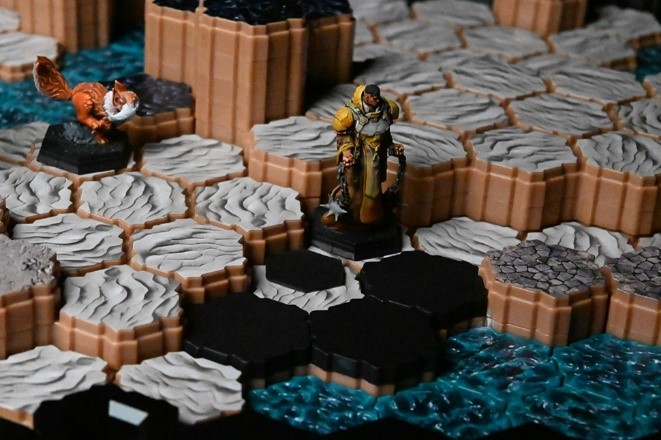
\includegraphics[width=1\linewidth]{chapters//Movement/TimeStrikeMovement1.jpg}
    \caption{This Character is going to move 3 hexes, denoted by the marked path.}
\end{figure}

\begin{figure}[h]
    \centering
    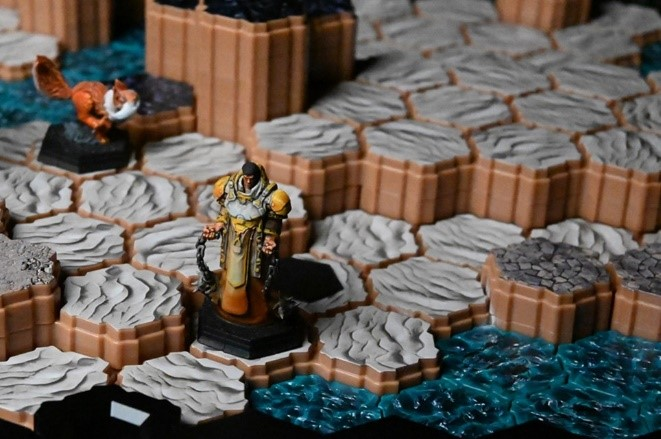
\includegraphics[width=1\linewidth]{chapters//Movement/TimeStrikeMovement2.jpg}
    \caption{The character used 3 movement to move a total of 3 hexes.}
\end{figure}

\subsection{Moving Multi-hex Units}
When moving a multi-hex unit with a base that takes up two or more hex spaces (also referred to as a 2-hex unit, 3- hex unit, etc.), decide which end to lead with - the front or the back. Then, move the unit so that the back end follows the same hexes that the leading end just left. When moving a multi-hex unit across uneven hexes, the unit must continue using its Movement until its base is able to rest completely on even hexes.
\textit{Note: Certain skills may allow Characters to flatten elevation when finishing a move.}

\subsection{Obstacles}
Units cannot move through enemy units, walls, Monsters, or other obstacles. The only thing they can move through it other units on their team if those units are not engaged. (See section on Engagement further down in this section.)

\section{Movement Penalties}
There are two types of Movement penalties: Swimming and Climbing. 
\subsection{Swimming}
Whenever a unit is on a water or liquid tile, they are considered to be swimming. Units that are swimming require one additional Movement to move between hexes. For instance, moving between two adjacent, same level water hexes uses a total of 2 Movement. Moving out of water (from water to land) also uses a total of 2 Movement. Moving into water (from land to water), does not use additinal movement and is not considered Swimming. 

\begin{figure}[h]
    \centering
    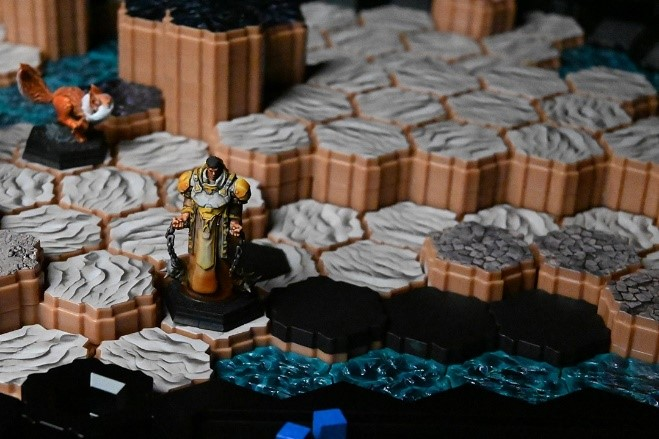
\includegraphics[width=1\linewidth]{chapters//Movement/TimeStrikeWaterMovement1.jpg}
\end{figure}

\begin{figure}[h]
    \centering
    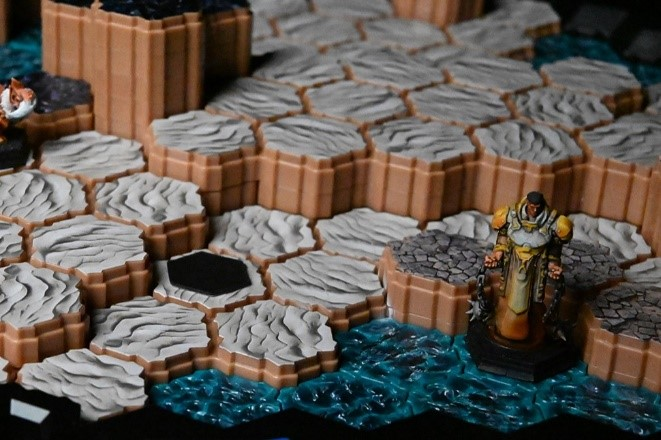
\includegraphics[width=1\linewidth]{chapters//Movement/TimeStrikeWaterMovement2.jpg}   
\end{figure}
In the picture example here, the Character has to use 4 Movement: 1 Movement to move to the adjacent land hex, 1 movement to enter the water hex, and 2 total Movement to move from one water hex to the next. 

\clearpage
\subsection{Climbing}
Climing is when a unit moves to a hex that is higher than the hex the unit is standing on. Count the difference in height between the two hexes to determine how much total Movement it will cost. Traversing to an adjacent hex that is one level higher than the starting location does not use any additional Movement. However, climbing two or more levels costs additional Movement, 1 level = 1 movement.

\begin{figure}[h]
    \centering
    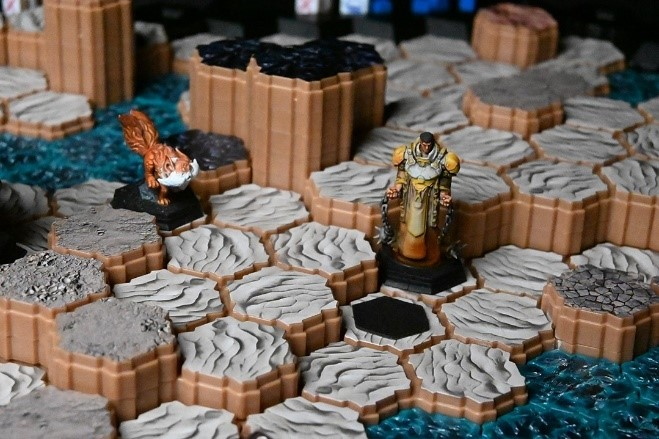
\includegraphics[width=0.75\linewidth]{chapters//Movement/TimeStrikeClimbing1.jpg}
\end{figure}

\begin{figure}[h]
    \centering
    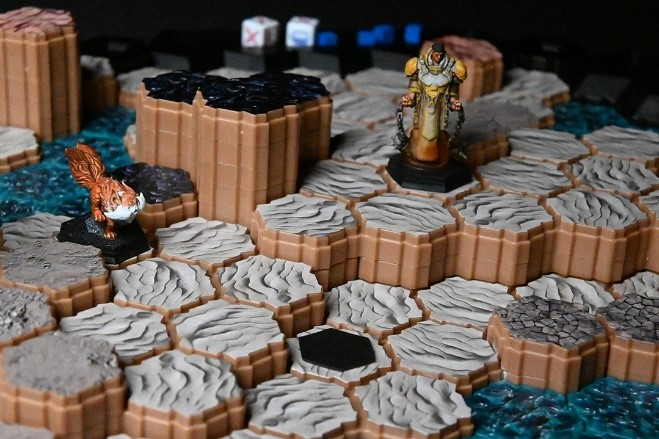
\includegraphics[width=0.75\linewidth]{chapters//Movement/TimeStrikeClimbing2.jpg}
\end{figure}

In this case, the Character used a total of 3 Movement. 2 hexes up for the climb and 1 hex forward.

\section{Movement Types}
All Characters in the game have specific Movement types found on their Character Card next to the Movement Stat. These include \textbf{Walk, Swim, or Fly}. Movement types can mitigate certain obstacles when moving. 

\textit{Note: If there is no Movement type listed next to the Movement stat, this means the default type is Walk. }
\subsection{Walk}
Walk is the most basic type of Movement and is subject to additional Movement costs such as swimming and climbing.

\subsection{Swim}
Swim allows a unit to ignore the Movement penalty for swimming. This means that that the units with the Swim Movement type do not use additional Movement when swimming. 

\subsection{Fly}
Fly allows a unit to ignore the Movement penalties for both swimming and climbing. Additionally, a unit with the Fly Movement type can move from one hex to another using only 1 Movement, regardless of any height difference between the hexes. They can also move over obstacles that typically block movement such as: enemy units, walls, and other obstacles. \textit{Note: Obstacles can only be moved over IF the character is able to end their Movement on an unoccupied hex} Units with the Fly Movement type are also never affected by fall damage during their own activation. Lastly, units with the Fly Movement type do not engage units when moving past them; engagement only happens once the Character stops moving.

\section{Falling}
Falling occurs when a unit moves down to a lower hex and the difference in height from its starting hex is greater than the height of the unit. Certain situations other than normal movement (such as Jump Attacks, being Contested, or pushed.) can also cause a unit to fall and take fall damage. 

\begin{figure}[h]
    \centering
    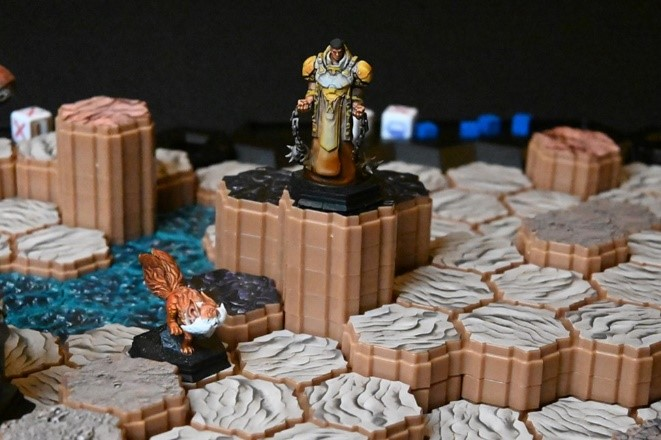
\includegraphics[width=0.85\linewidth]{chapters//Movement/TimeStrikeFallDamage.jpg}
\end{figure}

Example: A 4 height character is falling a total of 5 hexes. This will cause fall damage. 

\textbf{Exceptions:} Falling into water or moving along a road negates fall damage. Units with the Fly Movement type also ignore falling when moving during their own activation. 

\subsection{Taking Fall Damage}
For each hex greater than the falling unit's height, the player rolls one combat dice. One damage is taken for each Attack icon showing. \textit{Note: The amount of dice rolled for fall damage cannot exceed the unit's maximum health.}

Example: A unit has a height of 4, and they fall 6 hexes. They end up falling 2 hexes greater than their height, so 2 Combat Dice are rolled to determine fall damage. 
\begin{figure}[h]
    \centering
    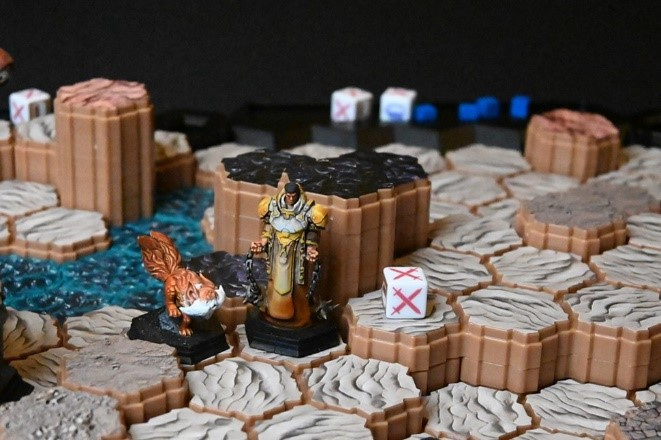
\includegraphics[width=0.85\linewidth]{chapters//Movement/TimeStrikeFallDamage2.jpg}
\end{figure}

\subsection{Getting Knocked off the Sentience}
Whenever a unit is knocked off the Sentience and is placed on a land hex, they must roll for 1 falling damage. 

\subsection{Falling from Destroyed Terrain}
Whenever a unit has moved because of land being destroyed, use the normal falling damage rules from their starting hex to their ending hex. 

\section{Roads}
A connected area of road hexes is called a road. Roads help units move around faster and allow them to ignore fall damage when moving along the road. A Character on a road hex may use 1 Movement to move and/or climb any distance along that road.

\textit{Note: Characters cannot move through enemy units while moving along the road.}

\section{Engagement}
Engagement is when two units belonging to different players (or the Lost) are adjacent to each other. This places both units into a state of engagement.

\textit{Exception: If units are adjacent to each other at different heights, the lowers units height value must be equal to or greater than the number of levels of elevation between the bases of the two units. If the hex height is greater than the lower unit’s height, those units are not engaged. }

\begin{figure}[h]
    \centering
    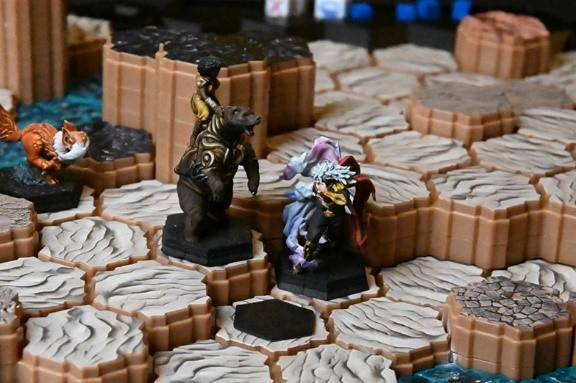
\includegraphics[width=1\linewidth]{chapters//Movement/TimeStrike2EngagedUnits.jpg}
\end{figure}

\subsection{Rules of Engagement}
When any number of enemy units are engaged with each other, they cannot target friendly or enemy units outside of that engagement. If they wish to target a unit they are not engaged with, they must leave the engagement. (See the rules for Targeting). 

\begin{figure}[h]
    \centering
    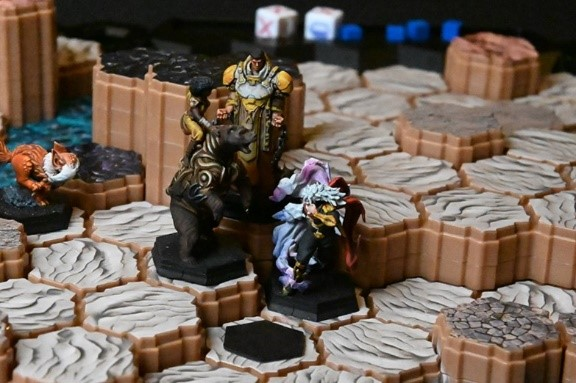
\includegraphics[width=1\linewidth]{chapters//Movement/TimeStrikeMultipleEngagedUnits.jpg}
\end{figure}

\subsection{Cheap Shot}
A Cheap Shot is a mechanic in which a unit rolls 1D6 for a chance of dealing one damage to another unit. This can be triggered by fleeing an engagement, Character skills, or various other situations. If the unit performing the Cheap Shot rolls an Attack icon, they deal 1 damage to the recipient of the Cheap Shot. Since a Cheap Shot is not an Attack Action, units cannot Defend against a Cheap Shot. Lost units never perform Cheap Shots unless they are controlled by a Myth (See the rules for Myths). ]

\subsection{Fleeing an Engagement}
Several situations allow units to perform Cheap Shots, but the primary situation occurs when a unit leaves an engagement. If an engaged unit leaves an engagement with an enemy unit controlled by another player by using its Movement stat to move away, it is considered to be fleeing the engagement and the enemy unit can perform a Cheap Shot against the fleeing unit. The Cheap Shot occurs immediately after the moving unit enters a hex in which they are not engaged with the enemy unit. If a unit flees engagement with multiple enemy units, each unit may perform a Cheap Shot against the fleeing unit. If the enemy units belong to multiple players, the Cheap Shots are performed in turn order.
\textit{Note: Since a unit is only fleeing an engagement if it uses its Movement stat to move away, a unit is not considered to be fleeing an engagement if it leaves by a Contest or Climb the Sentience Action, an Ability is cast on them, or loot is used to move them.}
\begin{figure}[h]
    \centering
    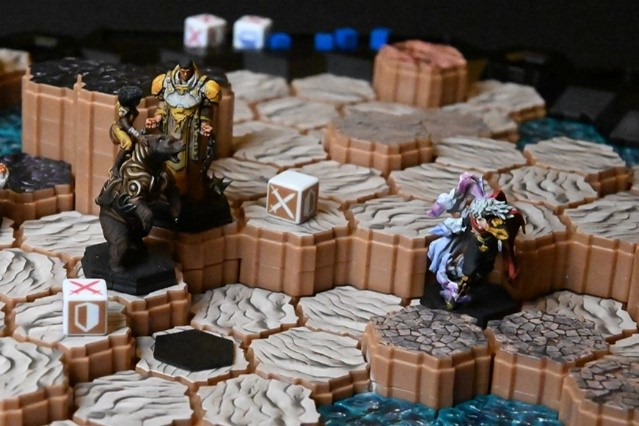
\includegraphics[width=1\linewidth]{chapters//Movement/TimeStrikeCharFleeingEngagement.jpg}
\end{figure}

Image: Character fleeing engagement with multiple units and one of them landing a successful Cheap Shot. 

\clearpage

\end{document}
